\documentclass[12pt]{article}
\usepackage{xeCJK}%preamble part
\usepackage{graphicx}
\usepackage{indentfirst}
\usepackage[a4paper, inner=1.5cm, outer=3cm, top=2cm, bottom=3cm, bindingoffset=1cm]{geometry}
\usepackage{epstopdf}
\usepackage{array}
\usepackage{fontspec}
\usepackage{gensymb}
\usepackage{amsmath}
\usepackage[citecolor=blue]{hyperref}

\usepackage{makecell}
\usepackage[lofdepth,lotdepth]{subfig}
\setCJKmainfont[BoldFont={SimHei}]{SimSun}
\setCJKmonofont{SimSun}
\setmainfont{Times New Roman}
\newCJKfontfamily[hei]\heiti{SimHei}
\setlength{\extrarowheight}{4pt}
\setlength{\parindent}{1cm}
\begin{document}
\title{\textbf{\fontsize{15.75pt}{\baselineskip}{模型的分析和仿真的结果}}} 

\author{\fontsize{12pt}{\baselineskip}{数33 赵丰}}
\maketitle
\large
\section{\textbf{\fontsize{12pt}{\baselineskip}{模型分析}}}
虽然RNA序列由于自身碱基配对而使得序列的相关性分析更复杂,但对于其中一小段较短的片段,可以近似认为其具有如下的单步转移概率矩阵:
\[
P=\left(
\begin{array}{cc}
p & 1-p \\
1-p & p
\end{array}
\right)
\]
其中p接近1.由转移矩阵P可以直接求出$R(1)=\frac{p}{2}$,其相关系数为$\rho(1)=\frac{R(1)-E(X_n)E(X_{n-1})}{\sigma_{X_n}^2}=2p-1$
$\rho(1)$接近1,表明相邻位点间的正相关系数接近1.类似的,可以求出n步相关系数为$\rho(n)=(2p-1)^n$,具体推导见附录1。
如果想利用相邻位点的相关性信息对某一个位点做估计,则对于给定的相关系数阀值$\alpha$,令$\rho(n)>\alpha$,解出最多可以利用的相邻位点数目
为$2n=\frac{2\log(alpha)}{\log(2p-1)}$
\section{\textbf{\fontsize{12pt}{\baselineskip}{仿真结果}}}
使用R语言产生一Markov Chain,其中p=0.95,由于过程平稳,可利用相关函数的遍历性质求出R(n)的样本值,将其与理论结果进行比较,作图如下:
\begin{figure}[!ht]
\centering
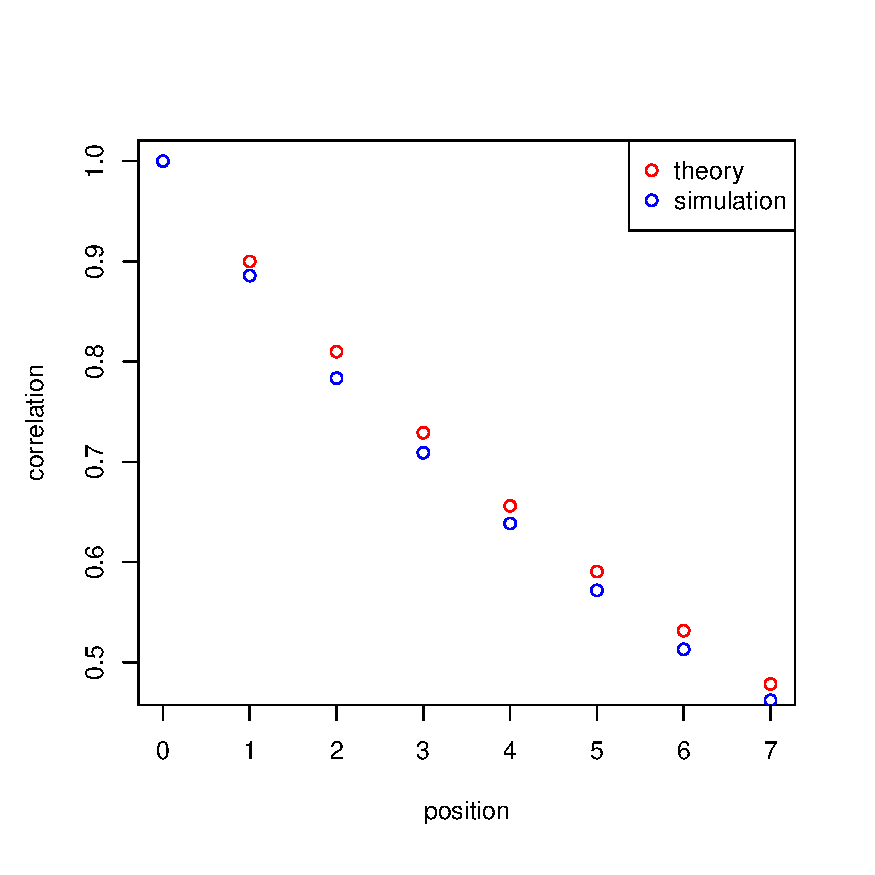
\includegraphics{Plotting1.eps}
\end{figure}
\newpage
\section{\textbf{\fontsize{12pt}{\baselineskip}{模型检验}}}
对于已知结构的RNA序列,试图求出p,使得均方误差$\sum_{k=1}^n ((2p-1)^k-\hat{R}(k))^2$最小,其中n取
$\lfloor \frac{\log(\alpha)}{\log(2p-1)} \rfloor$,其中$\alpha$事先给定。

实际对已知结构(链长为300)的某条RNA求相关系数发现$\hat{R}(1)=0.46$且当$n \ge 3$时$\hat{R}(n)\le 0$,这说明之前关于相邻链的相关性
的假定很可能是不正确的,需要寻找新的可以更好地推断原RNA二级结构的数学模型。
\section{\textbf{\fontsize{12pt}{\baselineskip}{Appendix 1:$\rho(n)$表达式的推导}}}
假设$X_0$服从Bernoulli 01分布,概率为$\frac{1}{2}$,记为行向量$\vec{p_0}=(\frac{1}{2},\frac{1}{2})$,第一个位置表示处于状态0的概率,
第二个位置表示处于状态1的概率。则$X_1$的分布为$\vec{p_0}=\vec{p_1}P=\vec{p_0}$,递推得到$X_n$的分布为与$\vec{p_0}$相同。在这种情形下,
$R(1)=P(X_n=1,X_{n-1}=1)=P(X_{n-1}=1)P(X_n=1|X_{n-1}=1)=\frac{p}{2}$。
为计算n步自相关函数,需要先求出n步转移矩阵$P^n$的表达式,为此可以采用特征值分解的方法,先将矩阵P分解为:
\[
P=Q\left(
\begin{array}{cc}
1 & 0 \\
0 & 2p-1
\end{array}
\right)Q^{-1},Q=\left(
\begin{array}{cc}
1 & 1 \\
1 & -1
\end{array}
\right)
\]
则\[
P^n=Q\left(
\begin{array}{cc}
1 & 0 \\
0 & (2p-1)^n
\end{array}
\right)Q^{-1}=
\left(
\begin{array}{cc}
\frac{1+(2p-1)^n}{2} & \frac{1-(2p-1)^n}{2} \\
\frac{1-(2p-1)^n}{2} & \frac{1+(2p-1)^n}{2}
\end{array}
\right)
\]
于是$R(n)=\frac{1+(2p-1)^n}{4},\rho(n)=\frac{R(n)-\frac{1}{4}}{\frac{1}{4}}=(2p-1)^n$
\section{\textbf{\fontsize{12pt}{\baselineskip}{参考文献}}}
\begin{thebibliography}{}
\bibitem{Bib1}    
 生物信息学
 
\end{thebibliography}
\end{document}